%!TEX root = ../TFM.tex
\chapter{Desarrollo extenso de la Unidad Didáctica}


\label{app:todo}

%%%%%%%%%%%%%%%%%%%%


Falta:

\begin{itemize}
	\item Incluir más cosas en la tienda.
	\item Definir los puntos que se obtienen por todo.
	%\item \hl{Estructura de inclusión de pdfs que mantenga la numeración y encabezado.}
	%\item \hl{Docu 1 de \Arab: Expresiones algebraicas y su valor numerico.}
	%\item Docu 2 de \Arab, cooperativo (multiplicación).
	%\item Docu 3 de \Arab, cooperativo (división).
	%\item Docu 4 de \Arab, individual unir-poli con factorización. Diseñado, hacer a mano.
	\item Docu Irresoluble de Ruffini.
	\item Reto final:
		\subitem Retos individuales.
		\subitem ¿Automatización del cambio de números?
		\subitem Parte cooperativa.
	\item Examen.
	\item Resumen, palabras clave.
	\item Abstract, key words.	
\end{itemize}

%%%%%%%%%%%%%%%%%%%

%\addcontentsline{toc}{chapter}{\protect\setcounter{tocdepth}{1}}

\settocdepth{section}

%%%%%%%%%%%%%%%%%%%%%%%%%%%%%%%%%%%%%%%%%%%%%%%%%%%%%%%%%%%%%%%%%%%
%%%%%%%%%%%%%%%%%%%%%%%%%%%%%%%%%%%%%%%%%%%%%%%%%%%%%%%%%%%%%%%%%%%
%%%%%%%%%%%%%% 			Sesión 0		%%%%%%%%%%%%%%%%%%%%%%%%%%%
%%%%%%%%%%%%%%%%%%%%%%%%%%%%%%%%%%%%%%%%%%%%%%%%%%%%%%%%%%%%%%%%%%%
%%%%%%%%%%%%%%%%%%%%%%%%%%%%%%%%%%%%%%%%%%%%%%%%%%%%%%%%%%%%%%%%%%%

\section{Sesión 0}


\paragraph{Contenidos}

Los contenidos a tratar en esta sección serán:

\begin{itemize}
\item Expresiones algebraicas.
\item Monomios y operaciones básicas.
\item Valor numérico.
\end{itemize}

\paragraph{Desarrollo de la sesión: }

En esta primera sesión introductoria se explicará la narrativa de la gamificación: 
%
los alumnos son investigadores que buscan desentrañar un misterio y para ello, a veces formarán equipos de investigación, otras veces trabajarán autónomamente.
%
El objetivo no será ganar y ser el primero en descubrirlo, sino que, como todos somos investigadores al servicio de la ciencia, queremos desentrañar la verdad y que todos la entendamos.
%
Se trata de colaborar.

El misterio a resolver tiene ya 10 siglos.
%
\Arab, nacido en el actual Irak, dejó un mapa y unos acertijos para desenterrar un tesoro que se dejó en Madrid.
%
Consideró que sólo un árabe que supiera de matemáticas tanto como él sería capaz de resolverlo.
%
Han pasado varios siglos y se cree que con los conocimientos actuales será posible resolverlo.
%
El descubrimiento del mapa y los acertijos es muy reciente, por eso todavía no se ha desenterrado el tesoro.

Se explicará también la gamificación y que para la evaluación de su labor como investigadores se utilizarán logros y medallas que podrán ir adquiriendo a medida que avancen la investigación y puntos de reputación, según las tareas que realicen.

Se comentará que habrá momentos en los que trabajar por grupos.
%
Estos grupos los habrá hecho el docente \crossref{(ver \ref{grupos})} y se les explicará que siempre que se vaya a trabajar en grupo, será en estos grupos.
%
Se procederá al listado de los grupos y sus miembros.

Finalizados los aspectos introductorios, lo primero es asegurar que los alumnos disponen de la competencia matemática suficiente para llevar a cabo la tarea encomendada.
%
Para ello se realizará en esta primera sesión una prueba de aptitud para la tarea.
%
Esta prueba de nivel competencial se realizará en el aula de informática con \textit{Kahoot}.
%
Servirá como repaso de los contenidos de otros años: expresiones algebraicas, operaciones con monomios, valor numérico.
%
Cada bloque de preguntas irá precedido de un pequeño vídeo que refresque los contenidos.
%
A los puntos otorgados por \textit{Kahoot} se le incorporará un bonus polinómico por preguntas acertadas para priorizar la precisión frente a la rapidez.
%
Los alumnos que la hayan superado obtendrán el logro de \logro{Investigador Apto}{investigador_apto}.
%
Los alumnos que no lo hayan superado en clase, tendrán la opción de repetir la prueba en casa para conseguir el logro de \ref{logro::investigador_apto}.


\subsection{Desarrollo del Kahoot}

El vídeo introductorio para el Kahoot será \cite{VideoKahootSes1}, por su buena y breve explicación sobre los temas que se trabajarán.
%
\todo{Definir puntos por pregunta}
%
El total de puntos que podrán conseguir será: 

aplicando el bonus.
\todo{bonus}

\newbloq Preguntas de 30 segundos.

\newpreg{\hl{0}}{Calcula.Identifica las expresiones algebraicas entre las siguientes:}

\begin{itemize}
\item \correcta{a)} $3x^3+2x^2y^3 + 7z$
\item b) $7·x^z$
\item \correcta{c)} $\frac{a^2b^3c^1}{c^6d^5}$
\item \correcta{d)} $7x^{15} + 15x^7 + 5x^{17}$
\item \correcta{e)} $7·x+9y = 5$
\end{itemize}


\newpreg{\hl{0}}{Calcula.Identifica monomios:}

\begin{itemize}
\item \correcta{a)} $x^7$
\item b) $4x^6+5x^3$
\item \correcta{c)} $5a^3b^2c^1$
\item d) $\frac{a^2b^3c^1}{c^6d^5}$
\item \correcta{e)} $\frac{7x^4}{4}$
\end{itemize}


\newpreg{\hl{0}}{Calcula.¿Cuál es el resultado de esta operación?}
\[
	7x^3+5x^3
\]

\begin{itemize}
	\item a) No se puede operar: $7x^3+5x^3$
	\item b) $12x^6$
	\item \correcta{c)} $12x^3$
	\item d) $35x^3$
	\item e) $35x^6$
\end{itemize}

\newpreg{\hl{0}}{Calcula.¿Cuál es el resultado de esta operación?}
\[
	7x^3+5x^2
\]

\begin{itemize}
	\item \correcta{a)}No se puede operar:  $7x^3+5x^2$
	\item b) $12x^5$
	\item c) $12(x^3+x^2)$
	\item d) $35x^3$
	\item e) $35x^6$
\end{itemize}

\newpreg{\hl{0}}{Calcula.¿Cuál es el resultado de esta operación?}
\[
	7x^3·5x^3
\]

\begin{itemize}
	\item a) No se puede operar: $7x^3+5x^3$
	\item b) $12x^6$
	\item c) $12x^3$
	\item d) $35x^3$
	\item \correcta{e)} $35x^6$
\end{itemize}


\newpreg{\hl{0}}{Calcula.¿Cuál es el resultado de esta operación?}
\[
	\frac{7(xy)^3}{5x^3}
\]

\begin{itemize}
	\item a) No se puede operar: $\frac{7(xy)^3}{5x^3}$
	\item \correcta{b)} $\rfrac{7y^3}{5}$
	\item c) $\frac{7y^3}{5x^2}$
	\item d) $35x^3$
	\item e) $35x^6$
\end{itemize}

\newpreg{\hl{0}}{Calcula.¿Cuál es el valor numérico de esta expresión para $a=3$ y $b=1$?}
\[
	\frac{7·b^{150}+a^2}{(a·b)^2}
\]

\begin{itemize}
	\item a) $7$
	\item \correcta{b)} $\frac{16}{9}$
	\item c) $\frac{5}{3}$
	\item d) $1$
	\item e) $15$
\end{itemize}

% 7 preguntas de 30 secs

\newbloq Preguntas de 1 minuto, 4 opciones:

\newpreg{\hl{0}}{Calcula.¿Cuál es el resultado de esta operación?}
\[
	7a^2b^3c^2 + 5a^2b^3c  + 7a^2bc^2 + 5a^2b^3c + 7a^2b^3c^2 + 5a^2b^3c 
\]

\begin{itemize}
	\item a) $12a^2b^3c + 12a^2bc^2$
	\item b) $36a^2b^3c^2$
	\item c) $10a^2b^3c^2 + 7a^2b^3c + 19a^2bc^2$
	\item \correcta{d)} $19a^2b^3c^2 + 10a^2b^3c + 7a^2bc^2$
\end{itemize}

\newpreg{\hl{0}}{Calcula.¿Cuál es el resultado de esta operación?}
\[
	2z^7 + 2·x^2 + y^6 + \frac{1}{2}x^2 - y^6 -z^7
\]

\begin{itemize}
	\item \correcta{a)} $z^7 + \rfrac{5}{2}x^2$
	\item b) $z^7 + \rfrac{3}{2}x^2 - 1$
	\item c) $z^7 + \rfrac{5}{2}x^2 - 1$
	\item d) $z^7 + \rfrac{3}{2}x^2$
\end{itemize}


\newpreg{\hl{0}}{Calcula.¿Cuál es el resultado de esta operación?}
\[
	3a^2b^3 · \rfrac{1}{3}a·b^3·c^2
\]

\begin{itemize}
	\item a) $a^3b^9c^2$
	\item b) $a^2b^9c^2$
	\item \correcta{c)} $a^3b^6c^2$
	\item d) $ac^2$
\end{itemize}


\newpreg{\hl{0}}{Calcula.¿Cuál es el resultado de esta operación?}
\[
	\frac{3x^2y^7z}{9xy^7z^2}
\]

\begin{itemize}
	\item \correcta{a)} $\frac{x}{3z}$
	\item b) No se puede operar porque quedaría una $z$ en el denominador.
	\item c) $0$
	\item d) $\frac{xy}{3z}$
\end{itemize}


\newpreg{\hl{0}}{Calcula.¿Cuál es el resultado de esta operación?}
\[
	\frac{4·a^2·x^7·b·x·a^3·y^4}{2·y^4·x^4·a}
\]

\begin{itemize}
	\item a) $2x^7a^2·b$
	\item b) $2a^5bx^2y$
	\item c) $\frac{2a^5bx^8y^4}{y^4x^4a}$
	\item \correcta{d)} $2a^4bx^4$
\end{itemize}


\newpreg{\hl{0}}{Calcula.\textit{Pregunta "trampa"} ¿Cuál es el valor numérico de esta expresión algebraica para $a=1$,$b=0$,$d=5$?}
\[
	\frac{4·a^2·c^7·b·d·a^3·c^4}{2·c^4·d^4·a}
\]

\begin{itemize}
	\item a) $2c^7a^2·b$
	\item \correcta{b)} $0$
	\item c) $\frac{2a^5bc^8d^4}{d^4c^4a}$
	\item d) No se puede calcular porque falta el valor de $c$
\end{itemize}

\newpreg{\hl{0}}{Calcula.¿Qué camino es más mejor para resolver el valor numérico de una expresión algebraica como podría ser la siguiente?}
\[
	\frac{4·a^2·c^7·b·d·a^3·c^4}{2·c^4·d^4·a}
\]

\begin{itemize}
	\item a) Sustituir todos los valores y operar.
	\item b) Operar algebraicamente y después sustituir los valores.
	\item c) Depende del caso.
	\item \correcta{d)} Depende del caso, pero en general la opción $b$ es correcta.
\end{itemize}

\newpreg{\hl{0}}{Calcula. ¿Cuál es el valor numérico de esta expresión algebraica para $x=-2$?}
\[
	\frac{2x^4-4x^2}{x^3+8}
\]

\begin{itemize}
	\item a) $1$.
	\item \correcta{b)} $0$.
	\item c) No existe.
	\item d) $2$.
\end{itemize}


%6 preguntas de 1 minuto.

\newbloq Bonus

\newpreg{\hl{0}}{Calcula.¿Es cierta esta igualdad?}
\[
	7x^3·x^{-2} \overset{?}{=} \frac{7x^3}{x^2} = 7x^{3-2} = 7x
\]

\begin{itemize}
	\item \correcta{a)} Sí.
	\item No.
\end{itemize}



%%%%%%%%%%%%%%%%%%%%%%%%%%%%%%%%%%%%%%%%%%%%%%%%%%%%%%%%%%%%%%%%%%%
%%%%%%%%%%%%%%%%%%%%%%%%%%%%%%%%%%%%%%%%%%%%%%%%%%%%%%%%%%%%%%%%%%%
%%%%%%%%%%%%%% 			Sesión 1		%%%%%%%%%%%%%%%%%%%%%%%%%%%
%%%%%%%%%%%%%%%%%%%%%%%%%%%%%%%%%%%%%%%%%%%%%%%%%%%%%%%%%%%%%%%%%%%
%%%%%%%%%%%%%%%%%%%%%%%%%%%%%%%%%%%%%%%%%%%%%%%%%%%%%%%%%%%%%%%%%%%

\section{Sesión 1}


\paragraph{Contenidos:}
Los contenidos a tratar en esta sesión son:
\begin{itemize}
\item Qué es un polinomio.
\item Grado de un polinomio.
\item Suma y diferencia de polinomios.
\item Producto de un monomio por un polinomio.
\item Factor común de monomios.
\end{itemize}


\paragraph{Desarrollo de la sesión} 

Se les entrega un supuesto \comillas{primer documento de \arab} (expuesto en \ref{app:DocModel}) en el que él mismo explica algunos conceptos.
%
Esta es una segunda prueba para comprobar que están a la altura del reto.
%
Este documento ya ha sido trabajado y resuelto, pero les puede servir para practicar antes de enfrentarse a los, todavía, irresolutos.
%
Durante la resolución del acertijo el docente paseará entre los alumnos resolviendo dudas y ayudando a quienes les esté costando más. 
%
Si resuelven con éxito este trabajo autónomo obtendrán el logro \logro{Investigador Nato}{investigador_nato}.
%
Si no lo han podido resolver en clase, será necesaria su resolución para la obtención del logro.

En caso de que el trabajo en clase se haya desarrollado satisfactoriamente y todos los alumnos hayan conseguido descifrar el acertijo, se propondrá un pequeño test online (\ref{test:ses1}) para seguir practicando y ejercitándose en el álgebra.
%
Excepcionalmente, en el caso de que el trabajo haya resultado muy complicado a los alumnos se podría emplear una sesión más en realizar los ejercicios del test en clase, con las explicaciones pertinentes del profesor.

Para la resolución de los ejercicios en casa dispondrán de la teoría y ejemplos resueltos en la ficha de trabajo del día además del libro de texto de apoyo ya mencionado.

Además, en esta sesión se pondrá en marcha el logro \logro{Contextualizador}{contextualizador}, que los alumnos podrán obtener por la aplicación de alguno de los contenidos de la clase de matemáticas en su vida cotidiana y su posterior explicación a la clase.

\subsection{Expresiones algebraicas y su valor numérico}
\label{app:DocModel}


\includepdf[pages=-,pagecommand={},width=1.22\textwidth]{pdf/RetoSes1.pdf}



\subsection{Test de la sesión 1}
\label{test:ses1}

\newbloq Test en edmodo sobre la suma y resta de polinomios

\newpreg{\hl{0}}{Sean $p(x) = x^2+5x-7$, $q(x) = x+7$ y $s(x) = -x^2-5x+7$. Calcula $p(x)+s(x)+2·q(x)$ y $p(x)-s(x)+q(x)$}


\newpreg{\hl{0}}{Multiplica $p(x) = -x^2+5$ por el monomio $-2x^2$}


\newpreg{\hl{0}}{Sea $p(x) = x^2+5x^6$, $q(y) = y^3+2y-15$. Calcula $s(z) = p(z)+q(z)$}

\newpreg{\hl{0}}{Sea $p(x) = x^2+5x^6$, $q(x) = x^3+2x-15$ y $s(x) = p(x) + q(x)$.
Calcula $p(2), q(2)$. Sin calcular s(2), ¿cuánto debería ser?}

\newpreg{\hl{0}}{Construye un polinomio de grado 2 con todos los términos, $p(x)$ , tal que $p(-2) = -6$}


\newcommand{\numpreg}

%%%%%%%%%%%%%%%%%%%%%%%%%%%%%%%%%%%%%%%%%%%%%%%%%%%%%%%%%%%%%%%%%%%
%%%%%%%%%%%%%%%%%%%%%%%%%%%%%%%%%%%%%%%%%%%%%%%%%%%%%%%%%%%%%%%%%%%
%%%%%%%%%%%%%% 			Sesión 2		%%%%%%%%%%%%%%%%%%%%%%%%%%%
%%%%%%%%%%%%%%%%%%%%%%%%%%%%%%%%%%%%%%%%%%%%%%%%%%%%%%%%%%%%%%%%%%%
%%%%%%%%%%%%%%%%%%%%%%%%%%%%%%%%%%%%%%%%%%%%%%%%%%%%%%%%%%%%%%%%%%%

\section{Sesión 2}



\paragraph{Contenidos}
\begin{itemize}
	\item Multiplicación de polinomios: propiedad asociativa y distributiva.
	\item Factor común de polinomios.
\end{itemize}

\paragraph{Desarrollo de la sesión}

Se les presentará el primer acertijo real irresoluto de la investigación.
%
Debido a la complejidad se trabajará por grupos.

Se les explicará a los alumnos que en cualquier trabajo siempre hay una fase previa de formación y para que puedan enfrentarse con alguna garantía al acertijo es necesario que conozcan algunas herramientas matemáticas, como la multiplicación de polinomios.
%
Se procederá a una explicación breve por parte del profesor en la pizarra sobre la multiplicación de polinomios explicando la propiedad asociativa y distributiva, incluyendo algunos ejemplos.

Una vez finalizada la explicación, se les entregará el acertijo expuesto en el anexo \ref{app:ses2:coop}
%
La resolución del acertijo es un número entero que corresponderá a la parte entera de la latitud del lugar en el que se escondió el tesoro.



Se les propondrá que realicen trabajo en casa para ejercitarse y poder resolver con garantías los siguientes retos.
%
Se les anunciará que para el próximo día se trabajará sobre un documento no resuelto a día de hoy y será necesario que dominen las matemáticas básicas que han aprendido en esta sesión.
%
Se les propondrán varios ejercicios en la plataforma online de los que tendrán que seleccionar un número determinado. 
%
En principio serían 3, pero este valor puede ser modificado dependiendo del desempeño de los alumnos durante la sesión.
%
Cada ejercicio tendrá asociado una puntuación: los ejercicios más difíciles otorgan más puntos, los ejercicios más fáciles, menos puntos.
%
Se especificará un número mínimo de puntos a conseguir para que los alumnos practiquen en casa. 
%
Para motivar que realicen los ejercicios, introducimos el logro \logro{Investigador Comprometido}{investigador_comprometido} nivel 1 que se obtiene si se obtiene el número de puntos mínimo\footnote{Los puntos correspondientes a la realización de los 3 ejercicios más fáciles}.
%
Podrán acceder al nivel 2 de este logro si realizan todos los ejercicios propuestos, aunque sólo recibirán puntos de 3 ejercicios.
%
Los ejercicios propuestos se encuentran en \ref{app:ses2:deberes}

\Justificacion{de la posibilidad de elección}
	%
	es bien sabido que los deberes no resultan motivadores para los alumnos. 
	%
	Para fomentar su realización se están utilizando 2 técnicas: 
	%
	la primera consiste en la explicación sobre la utilidad que puede tener para ellos (resolver mejor los próximos enigmas) y busca despertar una motivación intrínseca de competencia a corto plazo y no a largo plazo como tradicionalmente se hace (para hacer mejor el examen, para ser buen estudiante y tener un futuro asegurado, etc.).
	%
	Por otro lado, buscando fomentar su sentido de autonomía se les ofrece la posibilidad de elegir sobre los deberes a realizar. 
	%
	Pueden hacer un número variable de ejercicios dependiendo de su interés, habilidad y motivación.
	%
	Es importante la libertad de elección y que los jugadores sientan que esas elecciones son importantes \citep{werbach2012win}.

	Además, al ser resueltos en una plataforma online, son corregidos en el momento, provocando una retroalimentación sobre su desempeño inmediata
	%
	\footnote{Una posible mecánica de la gamificación según \citeauthor{werbach2012win}\crossref{, descrita en \ref{mecanicas}}.}.
	%
	Si los ejercicios propuestos suponen un desafío al alumno, se podría inducir un estado de flow llevando al alumno a querer resolver todos los ejercicios o por lo menos, a disfrutar durante su realización.


\subsection{Acertijo Cooperativo (sesión 2)}
\label{app:ses2:coop}

Se repartirá un documento por grupo. 
%
El documento para alumnos sólo contendrá rellenos los recuadros negros de texto blanco.
%
Los demás estarán vacíos y tendrán que rellenarlos.
%
Aquí se encuentran rellenos a modo de solucionario.

\includepdf[pages=-,pagecommand={},width=1.05\textheight,landscape=true]{pdf/RetoMulti.pdf}

\subsection{Deberes sesión 2}
\label{app:ses2:deberes}

\newbloq A realizar 3 de 5:

\newpreg{\hl{0}}{Sean 
$p(x) = 3x^2+5x+7$
y
$q(x) = -x^2+2$.
Calcula $p(x)·q(x)$
}

\newpreg{\hl{0}}{Sean 
$p(x) = -6x^6+18$
y
$q(x) = \frac{7}{6}x^4+x$.
Calcula $p(x)·q(x)$
}


\newpreg{\hl{0}}{Sean 
$p(x) = x^2+x+1$
y
$q(x) = x^4+x^3+x^2+x+1$.
Calcula $p(x)·q(x)$
}


\newpreg{\hl{0}}{Saca factor común todo lo que puedas en el polinomio
$p(x,y,z) = 3x^7y^2z + 9x^2y^2z + x^3y^2$
\textit{Sol: $3x^2y^2·(x^5z+3z+x) = 3x^2y^2·[z·(x^5+3)+x]$}
}

\newpreg{\hl{0}}{Sea $p(x) = x^2+5x^6$, $q(x) = x^3+2x-15$ y $s(x) = p(x) · q(x)$.
Calcula $p(2), q(2)$. Sin calcular s(2), ¿cuánto debería ser?}

%%%%%%%%%%%%%%%%%%%%%%%%%%%%%%%%%%%%%%%%%%%%%%%%%%%%%%%%%%%%%%%%%%%
%%%%%%%%%%%%%%%%%%%%%%%%%%%%%%%%%%%%%%%%%%%%%%%%%%%%%%%%%%%%%%%%%%%
%%%%%%%%%%%%%% 			Sesión 3		%%%%%%%%%%%%%%%%%%%%%%%%%%%
%%%%%%%%%%%%%%%%%%%%%%%%%%%%%%%%%%%%%%%%%%%%%%%%%%%%%%%%%%%%%%%%%%%
%%%%%%%%%%%%%%%%%%%%%%%%%%%%%%%%%%%%%%%%%%%%%%%%%%%%%%%%%%%%%%%%%%%

\section{Sesión 3}

\paragraph{Contenidos}
\begin{itemize}
	\item División de polinomios.
	\item Algoritmo de la división
\end{itemize}

\paragraph{Desarrollo de la sesión}

El desarrollo de esta sesión será el mismo que el de la sesión 2.
%
Una primera parte de exposición sobre el contenido necesario para la resolución del enigma y una ficha de trabajo cooperativo para su resolución que se encuentra en \ref{app:ses3:coop}.
%
El correcto resultado del acertijo les conducirá a otro número entero, que corresponderá a la parte entera de la longitud de la localización del tesoro.

Debido a que los alumnos desconocen que los 2 números enteros corresponden a la latitud y a la longitud, mediante un diálogo se les conducirá a esa conclusión.
%
Los conceptos de latitud y longitud se trabajan por primera vez en Ciencias Sociales de 1 de la ESO, según \bocm.


El trabajo a realizar en casa será encontrar la localización en un mapa de Madrid del recuadro que corresponde a la parte entera de la longitud y latitud.
%
Tendrán que saber qué número de los obtenidos corresponde a latitud y cuál a longitud.
%
Que impriman el mapa para pegarlo en su cuaderno de investigador.

\Justificacion{}
%
La realización de este ejercicio puede parecer que no trabaja la competencia matemática. 
%
Pero para la obtención del mapa es necesario tener claros los conceptos de parte entera y parte decimal.
%
Si la parte entera de la longitud es 3, la longitud real podría ser desde 3,01 hasta 3,99, lo que marca una gran diferencia.
%
Además, este ejercicio puede aumentar la involucración de los estudiantes en la narrativa de la gamificación y en el proceso.
%
Asimismo, supone un trabajo de la competencia digital (para encontrar el recuadro del mapa e imprimirlo).
%
Por otro lado, la división de polinomios se trabajará más adelante durante la unidad lo que permite aplazar la asimilación profunda del contenido.
%
Esta situación es diferente a la situación de la multiplicación de polinomios, ya que es una operación básica que deben interiorizar rápidamente ya que se utiliza para la división, para su posterior comprobación y para la factorización.
%
Por ello en la sesión de multiplicación es necesario trabajo en casa que trabaje el contenido, mientras que en la sesión de división no es imprescindible.


\subsection{Acertijo Cooperativo (sesión 3)}
\label{app:ses3:coop}

Este reto se realiza por parejas dentro del grupo.
%
Se repartirán 2 documentos por grupo y cada pareja trabajará independientemente. 
%
Así, cuando terminen podrán comparar resultados. 
%
En caso de que una pareja haya cometido algún error, la otra podrá ayudarles. 
%
De esta manera, podrán encontrar los errores con mayor rapidez y corregirlos adecuadamente.

Los 2 recuadros contienen la factorización de cada polinomio inicial.
%
Estos recuadros serán eliminados en el documento para los alumnos, pero sirven de solucionario para el docente.

\includepdf[pages=-,pagecommand={},width=1.05\textheight,landscape=true,clip,trim=80mm 0mm 20mm 50mm]{pdf/RetoDivision.pdf}



%%%%%%%%%%%%%%%%%%%%%%%%%%%%%%%%%%%%%%%%%%%%%%%%%%%%%%%%%%%%%%%%%%%
%%%%%%%%%%%%%%%%%%%%%%%%%%%%%%%%%%%%%%%%%%%%%%%%%%%%%%%%%%%%%%%%%%%
%%%%%%%%%%%%%% 			Sesión 4		%%%%%%%%%%%%%%%%%%%%%%%%%%%
%%%%%%%%%%%%%%%%%%%%%%%%%%%%%%%%%%%%%%%%%%%%%%%%%%%%%%%%%%%%%%%%%%%
%%%%%%%%%%%%%%%%%%%%%%%%%%%%%%%%%%%%%%%%%%%%%%%%%%%%%%%%%%%%%%%%%%%

\section{Sesión 4}


\paragraph{Contenidos}
\begin{itemize}
	\item Identidades notables: 
	\subitem Cuadrado de un binomio: $(x\pm a)^2 = \;x^2\pm 2xa + a^2$.
	\subitem Diferencia de cuadrados: $(x-a)(x+a) = x^2-a^2$.
\end{itemize}

\paragraph{Desarrollo de la sesión}

A quienes tengan el mapa en su cuaderno de investigador obtendrán un nivel más de su logro \ref{logro::investigador_comprometido}.

\Justificacion{} este ascenso inesperado es utilizado para transmitir el mensaje de que no todos los logros están sujetos a contingencias esperables que los alumnos conozcan.
%
En una buena gamificación también deben existir logros no sujetos a contingencias esperados. \citep{werbach2012win}.

Se propone para esta sesión que el docente diga que va a traer a un invitado especial a la clase de hoy.
%
Se dirá a los alumnos que el invitado que va a venir es un árabe de la escuela matemática de \arab y viene para enseñarles algunos contenidos específicos necesarios para la investigación y que él conoce a la perfección.
%
En realidad no habrá ningún invitado y se propone que simplemente sea el mismo docente disfrazado.
%
Esto será algo nuevo y muy llamativo que provocará una gran fijación en la memoria.
%
Podríamos conseguir lo que se denomina un \concept[Recuerdo Relámpago]{recuerdo relámpago}.
%f
Si todo sale según lo previsto, los alumnos recordarán toda su vida de la clase de matemáticas que les dio el docente disfrazado de árabe explicando las identidades notables, 
%
de una manera similar, en menor medida, a la que se grabó en la mente de muchas personas cuál era la actividad que estaban desarrollando con exactitud el día 11 de Septiembre de 2001 \citep{11s}.

Se empezará la sesión con un reto individual con el que podrán obtener puntos de reputación.
%
El docente tendría tiempo para disfrazarse mientras los alumnos se enfrentan al reto.
%
El reto consistirá en unir polinomios con su factorización (aunque todavía no sepan lo que es la factorización): lo harán multiplicando los paréntesis y uniendo con el polinomio correspondiente.
%
Aparecerán las 3 identidades notables varias veces para ir cogiendo soltura.
%
El reto se encuentra definido en el anexo \ref{app:ses4:indiv}.

Una vez finalizado el reto y otorgados los puntos, se procederá a una explicación en la pizarra sobre las identidades notables y su ámbito aplicación en todos los modos posibles:
%
para resolver multiplicaciones rápidamente, para resolver divisiones y para resolver ecuaciones.
%
Éste último punto servirá como introducción a la factorización.


Se propondrán ejercicios de deberes en \textit{edmodo} (ver \ref{ses4:deberes}) con el esquema utilizado anteriormente.


\subsection{Documentos para la sesión 4}

\subsubsection{Reto individual}
\label{app:ses4:indiv}

Se trata de unir cada producto de factores con su polinomio correspondiente. 
%
La solución es la siguiente:

\[
	\begin{array}{cc}
		(x-6)(x+1) & x^2-5x+6\\
		(x-3)(x-2)(x+4) & x^3-x^2-14x+24\\
		(x-2)(x+2) & x^2-4\\
		(x+3)^2 & x^2+6x+9\\
		(x-2)^2 & x^2-4x+4\\
		(x^2+1)(x-3) & x^3-3x^2+x-3\\
	\end{array}
\]


\begin{figure}[hbtp]
\centering
\caption{Trabajo autónomo de la sesión 4.}
\label{RetoUnir}
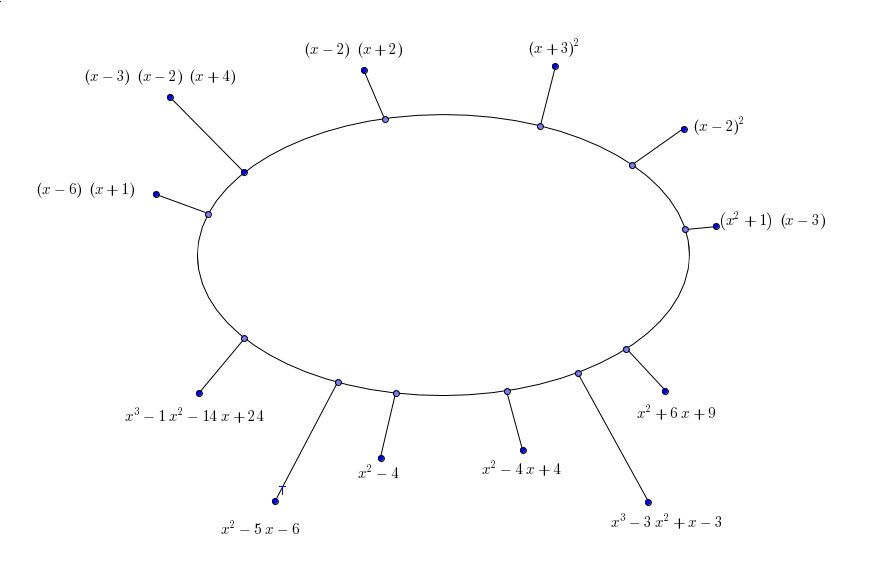
\includegraphics[scale=0.4]{img/RetoUnir.png}
\end{figure}


\subsubsection{Deberes}
\label{ses4:deberes}

\newbloq A realizar 4 de 6:

\newpreg{\hl{0}}{Calcula, sin multiplicar:
$(x-3)^2+(x+3)^2$
}

\newpreg{\hl{0}}{Calcula, sin multiplicar:
$-(x+3)^2+(x+3)(x-3) + 9$
}

\newpreg{\hl{0}}{Calcula, sin multiplicar:
$(-x+3)(-x-3)$
}

\newpreg{\hl{0}}{Calcula, sin multiplicar:
$(-x+3)^2+(-x+3)(-x-3) + 9$
}


\newpreg{\hl{0}}{Calcula, sin multiplicar:
$(x-3)^2+(x+3)^2$
}

\newpreg{\hl{0}}{Descompón la siguiente identidad notable: $x^2-2$
}

\newpreg{\hl{0}}{
	Descompón en un producto de identidades notables: $p(x) = x^4-16$
	\\\textit{Solución: $p(x) = (x^2+4)(x^2-4) = (x^2+4)(x+2)(x-2)$
	}
}



%%%%%%%%%%%%%%%%%%%%%%%%%%%%%%%%%%%%%%%%%%%%%%%%%%%%%%%%%%%%%%%%%%%
%%%%%%%%%%%%%%%%%%%%%%%%%%%%%%%%%%%%%%%%%%%%%%%%%%%%%%%%%%%%%%%%%%%
%%%%%%%%%%%%%% 			Sesión 5		%%%%%%%%%%%%%%%%%%%%%%%%%%%
%%%%%%%%%%%%%%%%%%%%%%%%%%%%%%%%%%%%%%%%%%%%%%%%%%%%%%%%%%%%%%%%%%%
%%%%%%%%%%%%%%%%%%%%%%%%%%%%%%%%%%%%%%%%%%%%%%%%%%%%%%%%%%%%%%%%%%%

\section{Sesión 5}


\paragraph{Contenidos}
\begin{itemize}
	\item Factorización. Conceptos teóricos, diferencia entre raíz y factor.
	\item Factorización utilizando: identidades notables, fórmula de resolución de ecuaciones de segundo grado, sacando factor común y aplicando los casos anteriores en polinomios de la forma: $P(x) = ax^3+bx^2+cx$.
\end{itemize}

\paragraph{Desarrollo de la sesión}

Se pone en marcha la medalla de \logro{Ojo Avizor}{avizor}.
%
Esta medalla tiene 3 subniveles y como máximo se puede ascender un nivel en cada clase.
%
Cada vez que en cualquier clase aparezca una identidad notable, cualquier alumno podrá levantar la mano para identificarla y resolverla. 
%
Si la resuelve correctamente obtendrá un subnivel del logro.

La sesión se desarrollará utilizando la exposición por parte del docente con abundantes ejemplos y ejercicios para practicar por parte de los alumnos.
%
La sesión comenzará enlazando con el final de la sesión anterior: utilización de identidades notables para encontrar los ceros un polinomio.
%
Se explicará que a estos ceros se les llama raíces y que con ellos se pueden construir factores para escribir el polinomio como un producto de términos de la forma $(x-a)$ con $a\in\real$.
%
A estos factores que se multiplican, se les llama factores y al proceso de escribir un polinomio como producto de sus factores se le denomina factorización.

A continuación se empleará todo el tiempo restante en factorizar polinomios.
%
El docente realizará primero uno utilizando un método (identidades notables) y se propondrá a los alumnos 2 polinomios para factorizar así.
%
Se realizará lo mismo con los otros 2 métodos: resolución de ecuaciones de segundo grado y factor común.

Se propone el siguiente itinerario:

\begin{itemize}
	\item Factorizar $x^4-16$. Proponer para factorizar $(x-3)·(x-2)$,$x^4-9 = (x^2+9)(x-\sqrt{3})(x+\sqrt{3})$ y $x^2+6x+9 = (x+3)^2$.
	
	\item Factorizar $x^2-5x+6$. Proponer para factorizar $x^2-2x-8 = (x-4)(x+2)$ y $2x^4-3x-2 = (2x+1)(x-2)$
	\item Factorizar $x^5-16x^3$. Proponer para factorizar $x^3-6x^2+9x = x(x-3)^2$.
	\item Si da tiempo: Factorizar $x^4+6x^2+9$. Proponer para factorizar $x^4-5x^2+6$.
\end{itemize}




%%%%%%%%%%%%%%%%%%%%%%%%%%%%%%%%%%%%%%%%%%%%%%%%%%%%%%%%%%%%%%%%%%%
%%%%%%%%%%%%%%%%%%%%%%%%%%%%%%%%%%%%%%%%%%%%%%%%%%%%%%%%%%%%%%%%%%%
%%%%%%%%%%%%%% 			Sesión 6		%%%%%%%%%%%%%%%%%%%%%%%%%%%
%%%%%%%%%%%%%%%%%%%%%%%%%%%%%%%%%%%%%%%%%%%%%%%%%%%%%%%%%%%%%%%%%%%
%%%%%%%%%%%%%%%%%%%%%%%%%%%%%%%%%%%%%%%%%%%%%%%%%%%%%%%%%%%%%%%%%%%

\section{Sesión 6}

\paragraph{Contenidos}
\begin{itemize}
	\item Algoritmo de factorización de Ruffini.
\end{itemize}

\paragraph{Desarrollo de la sesión}

Se les propondrá un reto cooperativo durante la primera media hora (ver \ref{ses6:coop}).
%
Este reto es muy completo y no lo conseguirán terminar porque incluirá una factorización de un polinomio de grado 4 y otro de grado 3 con término independiente.
%
Así, será necesario que escuchen e interioricen el método de Ruffini para factorizar polinomios.
%
Podrán practicar con los 2 polinomios del reto y con otros ejercicios propuestos por el docente con los que los alumnos podrán obtener puntos.
%
La resolución del reto correctamente les otorgará la parte decimal de la longitud de la localización del tesoro.

Se propondrán ejercicios de deberes en \textit{edmodo} (ver \ref{ses6:deberes}) con el esquema utilizado anteriormente.
%
En estos deberes se incorporará un vídeo con la explicación teórica sobre la factorización de polinomios con coeficiente principal distinto de 1.

\subsection{Reto cooperativo (sesión 6)}
\label{ses6:coop}

\subsubsection{Deberes}
\label{ses6:deberes}


\newbloq A elegir 3 de 6.

\newpreg{\hl{0}}{Factoriza, si es posible, $x^4+5x^3+5x^2-5x-6$.
\\\textit{Solución: $(x+2)(x+3)(x-1)(x+1)$
}
}

\newpreg{\hl{0}}{Factoriza, si es posible, $x^4+4x^3+6x^2-4x+1$.
\\\textit{Solución: $(x-1)^4$
}
}

\newpreg{\hl{0}}{Factoriza, si es posible, $x^2+x-42$.
\\\textit{Solución: $(x-6)(x+7)$}
}


\newpreg{\hl{0}}{Factoriza, si es posible, $x^4+x^3+x^2+x+1$.
\\\textit{No se puede factorizar.}
}

\newpreg{\hl{0}}{Factoriza, si es posible, $x^6-2x^3+1$.
\\\textit{Solución: $[(x-1)(x^2+x+1)]^2$}
}


\newpreg{\hl{0}}{Factoriza, si es posible, $x^{10}-4x^8+6x^6-4x^4+x^2$.
\\\textit{Solución: $x^2(x^2-1)^4$
}
}


%%%%%%%%%%%%%%%%%%%%%%%%%%%%%%%%%%%%%%%%%%%%%%%%%%%%%%%%%%%%%%%%%%%
%%%%%%%%%%%%%%%%%%%%%%%%%%%%%%%%%%%%%%%%%%%%%%%%%%%%%%%%%%%%%%%%%%%
%%%%%%%%%%%%%%\section 			y 8		%%%%%%%%%%%%%%%%%%%%%%%%%%%
%%%%%%%%%%%%%%%%%%%%%%%%%%%%%%%%%%%%%%%%%%%%%%%%%%%%%%%%%%%%%%%%%%%
%%%%%%%%%%%%%%%%%%%%%%%%%%%%%%%%%%%%%%%%%%%%%%%%%%%%%%%%%%%%%%%%%%%

\section{Sesiones 7 y 8}


\paragraph{Contenidos}
\begin{itemize}
	\item Repaso de todo, incluyendo la factorización de polinomios con coeficiente principal distinto de 1.
\end{itemize}

Se les entregará el último papiro sin resolver de la investigación para que lo resuelvan.
%
Es un reto complicado que implica aplicar con soltura todos los conocimientos aprendidos además de seguir aplicando conocimiento de años anteriores.


Se dispone de 2 sesiones para su realización: la primera se trabajará individualmente (cada miembro del equipo tendrá una ficha ligeramente diferente, ver \ref{ses7:indiv}) y la segunda se trabajará cooperativamente (ver \ref{ses7:coop}).
%
Para la segunda sesión será necesario que los alumnos hayan finalizado con éxito sus partes individuales, ya que el equipo necesitará los resultados obtenidos en la parte individual.

La correcta resolución del ejercicio cooperativo les dará la parte decimal de la latitud del lugar del tesoro.
%
En caso de que no les diera tiempo a resolverlo en clase, tendrían que terminarlo por su cuenta.

De cara a la preparación del examen tendrán en \textit{edmodo} un quizz que podrán hacer a modo de auto-evaluación cuantas veces quieran.

\subsection{Reto final (sesiones 7 y 8)}
\label{ses7:indiv}

\subsubsection{Alumno 1}

%!TEX root = ../TFM.tex

\subsubsection{Alumno 2}
%!TEX root = ../TFM.tex


\subsubsection{Alumno 3}
%!TEX root = ../TFM.tex


\subsubsection{Alumno 4}
%!TEX root = ../TFM.tex



\subsubsection{Parte cooperativa}
\label{ses7:coop}




%%%%%%%%%%%%%%%%%%%%%%%%%%%%%%%%%%%%%%%%%%%%%%%%%%%%%%%%%%%%%%%%%%%
%%%%%%%%%%%%%%%%%%%%%%%%%%%%%%%%%%%%%%%%%%%%%%%%%%%%%%%%%%%%%%%%%%%
%%%%%%%%%%%%%% 			Sesión 9		%%%%%%%%%%%%%%%%%%%%%%%%%%%
%%%%%%%%%%%%%%%%%%%%%%%%%%%%%%%%%%%%%%%%%%%%%%%%%%%%%%%%%%%%%%%%%%%
%%%%%%%%%%%%%%%%%%%%%%%%%%%%%%%%%%%%%%%%%%%%%%%%%%%%%%%%%%%%%%%%%%%

\section{Sesión 9}


En esta sesión, no necesariamente la sesión siguiente a la sesión 8, tendrá lugar el examen de la unidad (si se considera que haya un examen para esta unidad\crossref{, ver \ref{eval}}).
%
Los ejercicios propuestos para el examen se encuentran en \ref{examen}.


\subsection{Examen}
\label{examen}


\includepdf[pages=-,pagecommand={},width=1.22\textwidth]{pdf/Examen.pdf}


\subsection{Autoevaluación}
\label{app:autoeval}

Se propone para la autoevaluación del libro de apoyo \cite[p. 120]{MareaVerde} además de la realización de los ejercicios propuestos de deberes que no se hayan realizado a lo largo de la Unidad Didáctica.

\includepdf[pages={120},pagecommand={},width=1.2\textwidth]{pdf/3ESOBCompletoLOMCE.pdf}


